% ================================================================
% Chapter I/O & Diagnostics
% ================================================================
\chapter{Ouput and Diagnostics (IOM, DIA, TRD, FLO)}
\label{DIA}
\minitoc

\newpage
$\ $\newline    % force a new ligne

% ================================================================
%       Old Model Output 
% ================================================================
\section{Old Model Output (default or \key{dimgout})}
\label{DIA_io_old}

The model outputs are of three types: the restart file, the output listing, 
and the diagnostic output file(s). The restart file is used internally by the code when 
the user wants to start the model with initial conditions defined by a 
previous simulation. It contains all the information that is necessary in 
order for there to be no changes in the model results (even at the computer 
precision) between a run performed with several restarts and the same run 
performed in one step. It should be noted that this requires that the restart file 
contain two consecutive time steps for all the prognostic variables, and 
that it is saved in the same binary format as the one used by the computer 
that is to read it (in particular, 32 bits binary IEEE format must not be used for 
this file). 

The output listing and file(s) are predefined but should be checked 
and eventually adapted to the user's needs. The output listing is stored in 
the $ocean.output$ file. The information is printed from within the code on the 
logical unit $numout$. To locate these prints, use the UNIX command 
"\textit{grep -i numout}" in the source code directory.

By default, diagnostic output files are written in NetCDF format but an IEEE binary output format, called DIMG, can be choosen by defining \key{dimgout}. 

Since version 3.2, when defining \key{iomput}, an I/O server has been added which provides more flexibility in the choice of the fields to be written as well as how the writing work is distributed over the processors in massively parallel computing. The complete description of the use of this I/O server is presented in the next section. 

By default, if neither \key{iomput} nor \key{dimgout} are defined, NEMO produces NetCDF with the old IOIPSL library which has been kept for compatibility and its easy installation. However, the IOIPSL library is quite inefficient on parallel machines and, since version 3.2, many diagnostic options have been added presuming the use of \key{iomput}. The usefulness of the default IOIPSL-based option is expected to reduce with each new release. If \key{iomput} is not defined, output files and content are defined in the \mdl{diawri} module and contain mean (or instantaneous if \key{diainstant} is defined) values over a regular period of nn\_write time-steps (namelist parameter). 

%\gmcomment{                    % start of gmcomment

% ================================================================
% Diagnostics
% ================================================================
\section{Standard model Output (IOM)}
\label{DIA_iom}


Since version 3.2, iomput is the NEMO output interface of choice. It has been designed to be simple to use, flexible and efficient. The two main purposes of iomput are: 
\begin{enumerate}
\item The complete and flexible control of the output files through external XML files adapted by the user from standard templates. 
\item To achieve high performance and scalable output through the optional distribution of all diagnostic output related tasks to dedicated processes. 
\end{enumerate}
The first functionality allows the user to specify, without code changes or recompilation, aspects of the diagnostic output stream, such as:
\begin{itemize}
\item The choice of output frequencies that can be different for each file (including real months and years).
\item The choice of file contents; includes complete flexibility over which data are written in which files (the same data can be written in different files). 
\item The possibility to split output files at a choosen frequency.
\item The possibility to extract a vertical or an horizontal subdomain.
\item The choice of the temporal operation to perform, e.g.: average, accumulate, instantaneous, min, max and once.
\item Control over metadata via a large XML "database" of possible output fields.
\end{itemize}
In addition, iomput allows the user to add the output of any new variable (scalar, 2D or 3D) in the code in a very easy way. All details of iomput functionalities are listed in the following subsections. Examples of the XML files that control the outputs can be found in:
\begin{alltt}
\begin{verbatim}
  NEMOGCM/CONFIG/ORCA2_LIM/EXP00/iodef.xml
  NEMOGCM/CONFIG/SHARED/field_def.xml
  and
  NEMOGCM/CONFIG/SHARED/domain_def.xml.
\end{verbatim}
\end{alltt}

The second functionality targets output performance when running in parallel (\key{mpp\_mpi}). Iomput provides the possibility to specify N dedicated I/O processes (in addition to the NEMO processes) to collect and write the outputs. With an appropriate choice of N by the user, the bottleneck associated with the writing of the output files can be greatly reduced. 

In version 3.6, the iom\_put interface depends on an external code called \href{https://forge.ipsl.jussieu.fr/ioserver/browser/XIOS/branchs/xios-1.0}{XIOS-1.0} (use of revision 618 or higher is required). This new IO server can take advantage of the parallel I/O functionality of NetCDF4 to create a single output file and therefore to bypass the rebuilding phase. Note that writing in parallel into the same NetCDF files requires that your NetCDF4 library is linked to an HDF5 library that has been correctly compiled (i.e. with the configure option $--$enable-parallel). Note that the files created by iomput through XIOS are incompatible with NetCDF3. All post-processsing and visualization tools must therefore be compatible with NetCDF4 and not only NetCDF3.

Even if not using the parallel I/O functionality of NetCDF4, using N dedicated I/O servers, where N is typically much less than the number of NEMO processors, will reduce the number of output files created. This can greatly reduce the post-processing burden usually associated with using large numbers of NEMO processors. Note that for smaller configurations, the rebuilding phase can be avoided, even without a parallel-enabled NetCDF4 library, simply by employing only one dedicated I/O server.

\subsection{XIOS: the IO\_SERVER}

\subsubsection{Attached or detached mode?}

Iomput is based on \href{http://forge.ipsl.jussieu.fr/ioserver/wiki}{XIOS}, the io\_server developed by Yann Meurdesoif from IPSL. The behaviour of the io subsystem is controlled by settings in the external XML files listed above. Key settings in the iodef.xml file are {\tt using\_server} and the {\tt type} tag associated with each defined file. The {\tt using\_server} setting determines whether or not the server will be used in ''attached mode'' (as a library) [{\tt false}] or in ''detached mode'' (as an external executable on N additional, dedicated cpus) [{\tt true}]. The ''attached mode'' is simpler to use but much less efficient for massively parallel applications. The type of each file can be either ''multiple\_file'' or ''one\_file''.

In attached mode and if the type of file is ''multiple\_file'', then each NEMO process will also act as an IO server and produce its own set of output files. Superficially, this emulates the standard behaviour in previous versions, However, the subdomain written out by each process does not correspond to the {\tt jpi x jpj x jpk} domain actually computed by the process (although it may if {\tt jpni=1}). Instead each process will have collected and written out a number of complete longitudinal strips. If the ''one\_file'' option is chosen then all processes will collect their longitudinal strips and write (in parallel) to a single output file. 

In detached mode and if the type of file is ''multiple\_file'', then each stand-alone XIOS process will collect data for a range of complete longitudinal strips and write to its own set of output files. If the ''one\_file'' option is chosen then all XIOS processes will collect their longitudinal strips and write (in parallel) to a single output file. Note running in detached mode requires launching a Multiple Process Multiple Data (MPMD) parallel job. The following subsection provides a typical example but the syntax will vary in different MPP environments.

\subsubsection{Number of cpu used by XIOS in detached mode}

The number of cores used by the XIOS is specified when launching the model. The number of cores dedicated to XIOS should be from ~1/10 to ~1/50 of the number or cores dedicated to NEMO. Some manufacturers suggest using O($\sqrt{N}$) dedicated IO processors for N processors but this is a general recommendation and not specific to NEMO. It is difficult to provide precise recommendations because the optimal choice will depend on the particular hardware properties of the target system (parallel filesystem performance, available memory, memory bandwidth etc.) and the volume and frequency of data to be created. Here is an example of 2 cpus for the io\_server and 62 cpu for nemo using mpirun:

\texttt{ mpirun -np 62 ./nemo.exe : -np 2 ./xios\_server.exe }

\subsubsection{Control of XIOS: the XIOS context in iodef.xml}

As well as the {\tt using\_server} flag, other controls on the use of XIOS are set in the XIOS context in iodef.xml. See the XML basics section below for more details on XML syntax and rules.

\begin{tabular}{|p{4cm}|p{6.0cm}|p{2.0cm}|}
   \hline
   variable name & 
   description & 
   example \\ 
   \hline   
   \hline
   buffer\_size & 
   buffer size used by XIOS to send data from NEMO to XIOS. Larger is more efficient. Note that needed/used buffer sizes are summarized at the end of the job & 
   25000000 \\ 
   \hline   
   buffer\_server\_factor\_size & 
   ratio between NEMO and XIOS buffer size. Should be 2. & 
   2 \\ 
   \hline
   info\_level & 
   verbosity level (0 to 100) & 
   0 \\ 
   \hline
   using\_server & 
   activate attached(false) or detached(true) mode & 
   true \\ 
   \hline
   using\_oasis & 
   XIOS is used with OASIS(true) or not (false) & 
   false \\ 
   \hline
   oasis\_codes\_id & 
   when using oasis, define the identifier of NEMO in the namcouple. Note that the identifier of XIOS is xios.x & 
   oceanx \\ 
   \hline   
\end{tabular}


\subsection{Practical issues}

\subsubsection{Installation}

As mentioned, XIOS is supported separately and must be downloaded and compiled before it can be used with NEMO. See the installation guide on the \href{http://forge.ipsl.jussieu.fr/ioserver/wiki}{XIOS} wiki for help and guidance. NEMO will need to link to the compiled XIOS library. The 
\href{http://www.nemo-ocean.eu/Using-NEMO/User-Guides/Basics/XIOS-IO-server-installation-and-use}{XIOS with NEMO} guide provides an example illustration of how this can be achieved.

\subsubsection{Add your own outputs}

It is very easy to add your own outputs with iomput. Many standard fields and diagnostics are already prepared (i.e., steps 1 to 3 below have been done) and simply need to be activated by including the required output in a file definition in iodef.xml (step 4). To add new output variables, all 4 of the following steps must be taken.
\begin{description}
\item[1.] in NEMO code, add a \\
\texttt{      CALL iom\_put( 'identifier', array ) } \\
where you want to output a 2D or 3D array.

\item[2.] If necessary, add \\
\texttt{   USE iom\ \ \ \ \ \ \ \ \ \ \ \ ! I/O manager library }  \\
to the list of used modules in the upper part of your module. 

\item[3.] in the field\_def.xml file, add the definition of your variable using the same identifier you used in the f90 code (see subsequent sections for a details of the XML syntax and rules). For example:
\vspace{-20pt}
\begin{alltt}  {{\scriptsize
\begin{verbatim}
   <field_definition>
      <!-- T grid -->

     <field_group id="grid_T" grid_ref="grid_T_3D">
      ...
      <field id="identifier" long_name="blabla" ... />   
      ...
   </field_definition> 
\end{verbatim}
}}\end{alltt} 
Note your definition must be added to the field\_group whose reference grid is consistent with the size of the array passed to iomput. The grid\_ref attribute refers to definitions set in iodef.xml which, in turn, reference grids and axes either defined in the code (iom\_set\_domain\_attr and iom\_set\_axis\_attr in iom.F90) or defined in the domain\_def.xml file. E.g.:
\vspace{-20pt}
\begin{alltt}  {{\scriptsize
\begin{verbatim}
     <grid id="grid_T_3D" domain_ref="grid_T" axis_ref="deptht"/>
\end{verbatim}
}}\end{alltt} 
Note, if your array is computed within the surface module each nn\_fsbc time\_step, 
add the field definition within the field\_group defined with the id ''SBC'': $<$field\_group id=''SBC''...$>$ which has been defined with the correct frequency of operations (iom\_set\_field\_attr in iom.F90)

\item[4.] add your field in one of the output files defined in iodef.xml (again see subsequent sections for syntax and rules)   \\
\vspace{-20pt}
\begin{alltt}  {{\scriptsize
\begin{verbatim}
   <file id="file1" .../>   
      ...
      <field field_ref="identifier" />   
      ...
   </file>   
\end{verbatim}
}}\end{alltt} 

\end{description}
\subsection{XML fundamentals}

\subsubsection{ XML basic rules}

XML tags begin with the less-than character ("$<$") and end with the greater-than character (''$>$''). 
You use tags to mark the start and end of elements, which are the logical units of information 
in an XML document. In addition to marking the beginning of an element, XML start tags also 
provide a place to specify attributes. An attribute specifies a single property for an element, 
using a name/value pair, for example: $<$a b="x" c="y" b="z"$>$ ... $<$/a$>$.
See \href{http://www.xmlnews.org/docs/xml-basics.html}{here} for more details.

\subsubsection{Structure of the xml file used in NEMO}

The XML file used in XIOS is structured by 7 families of tags: context, axis, domain, grid, field, file and variable. Each tag family has hierarchy of three flavors (except for context):
\\
\begin{tabular}{|p{3.0cm}|p{4.5cm}|p{4.5cm}|}
   \hline
   flavor &
   description &
   example \\
   \hline
   \hline
   root &
   declaration of the root element that can contain element groups or elements &
   {\scriptsize \verb? < file_definition ... >?} \\
   \hline
   group &
   declaration of a group element that can contain element groups or elements &
   {\scriptsize \verb? < file_group ... >?} \\
   \hline
   element &
   declaration of an element that can contain elements &
   {\scriptsize \verb? < file ... >?} \\
   \hline
\end{tabular}
\\

Each element may have several attributes. Some attributes are mandatory, other are optional but have a default value and other are are completely optional. Id is a special attribute used to identify an element or a group of elements. It must be unique for a kind of element. It is optional, but no reference to the corresponding element can be done if it is not defined.

The XML file is split into context tags that are used to isolate IO definition from different codes or different parts of a code. No interference is possible between 2 different contexts. Each context has its own calendar and an associated timestep. In NEMO, we used the following contexts (that can be defined in any order):\\
\\
\begin{tabular}{|p{3.0cm}|p{4.5cm}|p{4.5cm}|}
   \hline
   context &
   description &
   example \\
   \hline
   \hline
   context xios &
   context containing information for XIOS &
   {\scriptsize \verb? <context id="xios" ...  ?} \\
   \hline
   context nemo &
   context containing IO information for NEMO (mother grid when using AGRIF) &
   {\scriptsize \verb? <context id="nemo" ... ?} \\
   \hline
   context 1\_nemo &
   context containing IO information for NEMO child grid 1 (when using AGRIF) &
   {\scriptsize \verb? <context id="1_nemo" ...  ?} \\
   \hline
   context n\_nemo &
   context containing IO information for NEMO child grid n (when using AGRIF) &
   {\scriptsize \verb? <context id="n_nemo" ...  ?} \\
   \hline
\end{tabular}
\\

\noindent The xios context contains only 1 tag:
\\
\begin{tabular}{|p{3.0cm}|p{4.5cm}|p{4.5cm}|}
   \hline
   context tag &
   description &
   example \\
   \hline
   \hline
   variable\_definition &
   define variables needed by XIOS. This can be seen as a kind of namelist for XIOS. &
   {\scriptsize \verb? <variable_definition ... ?} \\
   \hline
\end{tabular}
\\

\noindent Each context tag related to NEMO (mother or child grids) is divided into 5 parts (that can be defined in any order):\\
\\
\begin{tabular}{|p{3.0cm}|p{4.5cm}|p{4.5cm}|}
   \hline
   context tag &
   description &
   example \\
   \hline
   \hline
   field\_definition &
   define all variables that can potentially be outputted &
   {\scriptsize \verb? <field_definition ... ?} \\
   \hline
   file\_definition &
   define the netcdf files to be created and the variables they will contain &
   {\scriptsize \verb? <file_definition ... ?} \\
   \hline
   axis\_definition &
   define vertical axis &
   {\scriptsize \verb? <axis_definition ... ?} \\
   \hline
   domain\_definition &
   define the horizontal grids &
   {\scriptsize \verb? <domain_definition ... ?} \\
   \hline
   grid\_definition &
   define the 2D and 3D grids (association of an axis and a domain) &
   {\scriptsize \verb? <grid_definition ... ?} \\
   \hline
\end{tabular}
\\

\subsubsection{Nesting XML files}

The XML file can be split in different parts to improve its readability and facilitate its use. The inclusion of XML files into the main XML file can be done through the attribute src: \\
{\scriptsize \verb? <context src="./nemo_def.xml" /> ?}\\
 
\noindent In NEMO, by default, the field and domain definition is done in 2 separate files:
{\scriptsize \tt
\begin{verbatim}
NEMOGCM/CONFIG/SHARED/field_def.xml
and
NEMOGCM/CONFIG/SHARED/domain_def.xml 
\end{verbatim}
}
\noindent that are included in the main iodef.xml file through the following commands: \\
{\scriptsize \verb? <field_definition src="./field_def.xml" /> ? \\
\verb? <domain_definition src="./domain_def.xml" /> ? }


\subsubsection{Use of inheritance}

XML extensively uses the concept of inheritance. XML has a tree based structure with a parent-child oriented relation: all children inherit attributes from parent, but an attribute defined in a child replace the inherited attribute value. Note that the special attribute ''id'' is never inherited.  \\
\\
example 1: Direct inheritance.
\vspace{-20pt}
\begin{alltt}  {{\scriptsize    
\begin{verbatim}
   <field_definition operation="average" >
     <field id="sst"                    />   <!-- averaged      sst --> 
     <field id="sss" operation="instant"/>   <!-- instantaneous sss --> 
   </field_definition> 
\end{verbatim}
}}\end{alltt} 

The field ''sst'' which is part (or a child) of the field\_definition will inherit the value ''average'' 
of the attribute ''operation'' from its parent. Note that a child can overwrite 
the attribute definition inherited from its parents. In the example above, the field ''sss'' will 
for example output instantaneous values instead of average values. \\
\\
example 2: Inheritance by reference.
\vspace{-20pt}
\begin{alltt}  {{\scriptsize
\begin{verbatim}
   <field_definition>
     <field id="sst" long_name="sea surface temperature" />   
     <field id="sss" long_name="sea surface salinity"    />  
   </field_definition>      

   <file_definition>
     <file id="myfile" output_freq="1d" />   
       <field field_ref="sst"                            />  <!-- default def -->
       <field field_ref="sss" long_name="my description" />  <!-- overwrite   -->
     </file>   
   </file_definition> 
\end{verbatim}
}}\end{alltt} 
Inherit (and overwrite, if needed) the attributes of a tag you are refering to.

\subsubsection{Use of Groups}

Groups can be used for 2 purposes. Firstly, the group can be used to define common attributes to be shared by the elements of the group through inheritance. In the following example, we define a group of field that will share a common grid ''grid\_T\_2D''. Note that for the field ''toce'', we overwrite the grid definition inherited from the group by ''grid\_T\_3D''.
\vspace{-20pt}
\begin{alltt}  {{\scriptsize
\begin{verbatim}
   <field_group id="grid_T" grid_ref="grid_T_2D">
    <field id="toce" long_name="temperature"             unit="degC" grid_ref="grid_T_3D"/>
    <field id="sst"  long_name="sea surface temperature" unit="degC"                     />
    <field id="sss"  long_name="sea surface salinity"    unit="psu"                      />
    <field id="ssh"  long_name="sea surface height"      unit="m"                        />
         ...
\end{verbatim}
}}\end{alltt} 

Secondly, the group can be used to replace a list of elements. Several examples of groups of fields are proposed at the end of the file {\tt CONFIG/SHARED/field\_def.xml}. For example, a short list of the usual variables related to the U grid:
\vspace{-20pt}
\begin{alltt}  {{\scriptsize
\begin{verbatim}
   <field_group id="groupU" >
    <field field_ref="uoce"  />
    <field field_ref="suoce" />
    <field field_ref="utau"  />
   </field_group>
\end{verbatim}
}}\end{alltt} 
that can be directly included in a file through the following syntax:
\vspace{-20pt}
\begin{alltt}  {{\scriptsize
\begin{verbatim}
   <file id="myfile_U" output_freq="1d" />   
    <field_group group_ref="groupU"/>  
    <field field_ref="uocetr_eff"  />  <!-- add another field -->
   </file>   
\end{verbatim}
}}\end{alltt} 

\subsection{Detailed functionalities }

The file {\tt NEMOGCM/CONFIG/ORCA2\_LIM/iodef\_demo.xml} provides several examples of the use of the new functionalities offered by the XML interface of XIOS. 

\subsubsection{Define horizontal subdomains}
Horizontal subdomains are defined through the attributs zoom\_ibegin, zoom\_jbegin, zoom\_ni, zoom\_nj of the tag family domain. It must therefore be done in the domain part of the XML file. For example, in {\tt CONFIG/SHARED/domain\_def.xml}, we provide the following example of a definition of a 5 by 5 box with the bottom left corner at point (10,10).
\vspace{-20pt}
\begin{alltt}  {{\scriptsize
\begin{verbatim}
   <domain_group id="grid_T">
    <domain id="myzoom" zoom_ibegin="10" zoom_jbegin="10" zoom_ni="5" zoom_nj="5" />
\end{verbatim}
}}\end{alltt} 
The use of this subdomain is done through the redefinition of the attribute domain\_ref of the tag family field. For example:
\vspace{-20pt}
\begin{alltt}  {{\scriptsize
\begin{verbatim}
   <file id="myfile_vzoom" output_freq="1d" >
      <field field_ref="toce" domain_ref="myzoom"/>
   </file>
\end{verbatim}
}}\end{alltt} 
Moorings are seen as an extrem case corresponding to a 1 by 1 subdomain. The Equatorial section, the TAO, RAMA and PIRATA moorings are alredy registered in the code and can therefore be outputted without taking care of their (i,j) position in the grid. These predefined domains can be activated by the use of specific domain\_ref: ''EqT'', ''EqU'' or ''EqW'' for the equatorial sections and the mooring position for TAO, RAMA and PIRATA followed by ''T'' (for example: ''8s137eT'', ''1.5s80.5eT'' ...)
\vspace{-20pt}
\begin{alltt}  {{\scriptsize
\begin{verbatim}
   <file id="myfile_vzoom" output_freq="1d" >
      <field field_ref="toce" domain_ref="0n180wT"/>
   </file>
\end{verbatim}
}}\end{alltt} 
Note that if the domain decomposition used in XIOS cuts the subdomain in several parts and if you use the ''multiple\_file'' type for your output files, you will endup with several files you will need to rebuild using unprovided tools (like ncpdq and ncrcat, \href{http://nco.sourceforge.net/nco.html#Concatenation}{see nco manual}). We are therefore advising to use the ''one\_file'' type in this case.

\subsubsection{Define vertical zooms}
Vertical zooms are defined through the attributs zoom\_begin and zoom\_end of the tag family axis. It must therefore be done in the axis part of the XML file. For example, in NEMOGCM/CONFIG/ORCA2\_LIM/iodef\_demo.xml, we provide the following example:
\vspace{-20pt}
\begin{alltt}  {{\scriptsize
\begin{verbatim}
   <axis_group id="deptht" long_name="Vertical T levels" unit="m" positive="down" >
      <axis id="deptht" />
      <axis id="deptht_myzoom" zoom_begin="1" zoom_end="10" />
\end{verbatim}
}}\end{alltt} 
The use of this vertical zoom is done through the redefinition of the attribute axis\_ref of the tag family field. For example:
\vspace{-20pt}
\begin{alltt}  {{\scriptsize
\begin{verbatim}
   <file id="myfile_hzoom" output_freq="1d" >
      <field field_ref="toce" axis_ref="deptht_myzoom"/>
   </file>
\end{verbatim}
}}\end{alltt} 

\subsubsection{Control of the output file names}

The output file names are defined by the attributs ''name'' and ''name\_suffix'' of the tag family file. for example:
\vspace{-20pt}
\begin{alltt}  {{\scriptsize
\begin{verbatim}
   <file_group id="1d" output_freq="1d" name="myfile_1d" > 
      <file id="myfileA" name_suffix="_AAA" > <!-- will create file "myfile_1d_AAA"  -->
         ...
      </file>
      <file id="myfileB" name_suffix="_BBB" > <!-- will create file "myfile_1d_BBB" -->
         ...
      </file>
   </file_group>
\end{verbatim}
}}\end{alltt} 
However it is often very convienent to define the file name with the name of the experiment, the output file frequency and the date of the beginning and the end of the simulation (which are informations stored either in the namelist or in the XML file). To do so, we added the following rule: if the id of the tag file is ''fileN''(where N = 1 to 999 on 1 to 3 digits) or one of the predefined sections or moorings (see next subsection), the following part of the name and the name\_suffix (that can be inherited) will be automatically replaced by:\\
\\
\begin{tabular}{|p{4cm}|p{8cm}|}
   \hline
   \centering placeholder string & automatically  replaced by \\
   \hline
   \hline
   \centering @expname@ &
   the experiment name (from cn\_exp in the namelist) \\
   \hline
   \centering @freq@ &
   output frequency (from attribute output\_freq) \\
   \hline
   \centering @startdate@  &
   starting date of the simulation (from nn\_date0 in the restart or the namelist). \verb?yyyymmdd? format \\
   \hline
   \centering @startdatefull@  & 
   starting date of the simulation (from nn\_date0 in the restart or the namelist). \verb?yyyymmdd_hh:mm:ss? format \\
   \hline
   \centering @enddate@  &
   ending date of the simulation (from nn\_date0 and nn\_itend in the namelist). \verb?yyyymmdd? format \\
   \hline
   \centering @enddatefull@  & 
   ending date of the simulation (from nn\_date0 and nn\_itend in the namelist). \verb?yyyymmdd_hh:mm:ss? format \\
   \hline
\end{tabular}\\
\\

\noindent For example, 
{{\scriptsize
\begin{verbatim}
   <file id="myfile_hzoom" name="myfile_@expname@_@startdate@_freq@freq@" output_freq="1d" >
\end{verbatim}
}}
\noindent with the namelist:
{{\scriptsize
\begin{verbatim}
   cn_exp      =  "ORCA2"
   nn_date0    =  19891231
   ln_rstart   = .false.
\end{verbatim}
}}
\noindent will give the following file name radical:
{{\scriptsize
\begin{verbatim}
   myfile_ORCA2_19891231_freq1d 
\end{verbatim}
}}

\subsubsection{Other controls of the xml attributes from NEMO}

The values of some attributes are defined by subroutine calls within NEMO (calls to iom\_set\_domain\_attr, iom\_set\_axis\_attr and iom\_set\_field\_attr in iom.F90). Any definition given in the xml file will be overwritten. By convention, these attributes are defined to ''auto'' (for string) or ''0000'' (for integer) in the xml file (but this is not necessary). 

Here is the list of these attributes:\\
\\
\begin{tabular}{|l|c|c|c|}
   \hline
 \multicolumn{2}{|c|}{tag ids affected by automatic           }  & name      & attribute value \\
  \multicolumn{2}{|c|}{definition of some of their attributes }  & attribute  &        \\
   \hline
   \hline
    \multicolumn{2}{|c|}{field\_definition} & freq\_op & \np{rn\_rdt} \\
   \hline
    \multicolumn{2}{|c|}{SBC}               & freq\_op & \np{rn\_rdt} $\times$ \np{nn\_fsbc}  \\
   \hline
    \multicolumn{2}{|c|}{ptrc\_T}           & freq\_op & \np{rn\_rdt} $\times$ \np{nn\_dttrc} \\
   \hline
    \multicolumn{2}{|c|}{diad\_T}           & freq\_op & \np{rn\_rdt} $\times$ \np{nn\_dttrc} \\
   \hline
    \multicolumn{2}{|c|}{EqT, EqU, EqW} & jbegin, ni,      & according to the grid    \\
    \multicolumn{2}{|c|}{                         } & name\_suffix &                                      \\
   \hline
   \multicolumn{2}{|c|}{TAO, RAMA and PIRATA moorings} & zoom\_ibegin, zoom\_jbegin, & according to the grid    \\
    \multicolumn{2}{|c|}{                                                       } & name\_suffix &                                      \\
   \hline
\end{tabular}

\subsubsection{Advanced use of XIOS functionalities}

\subsection{XML reference tables}
\label{IOM_xmlref}

(1) Simple computation: directly define the computation when refering to the variable in the file definition.

\vspace{-20pt}
\begin{alltt}  {{\scriptsize    
\begin{verbatim}
 <field field\_ref="sst"  name="tosK"  unit="degK" > sst + 273.15 </field>
 <field field\_ref="taum" name="taum2" unit="N2/m4" long\_name="square of wind stress module" > taum * taum </field>
 <field field\_ref="qt"   name="stupid\_check" > qt - qsr - qns </field>
\end{verbatim}
}}\end{alltt} 

(2) Simple computation: define a new variable and use it in the file definition.

in field\_definition:
\vspace{-20pt}
\begin{alltt}  {{\scriptsize    
\begin{verbatim}
 <field id="sst2" long\_name="square of sea surface temperature" unit="degC2" >  sst * sst </field >
\end{verbatim}
}}\end{alltt} 
in file\_definition:
\vspace{-20pt}
\begin{alltt}  {{\scriptsize    
\begin{verbatim}
 <field field\_ref="sst2" > sst2 </field>
\end{verbatim}
}}\end{alltt} 
Note that in this case, the following syntaxe $<$field field\_ref="sst2" /$>$ is not working as sst2 won't be evaluated.

(3) Change of variable precision:

\vspace{-20pt}
\begin{alltt}  {{\scriptsize    
\begin{verbatim}
     <!-- force to keep real 8 -->
 <field field\_ref="sst" name="tos\_r8" prec="8" />
      <!-- integer 2  with add\_offset and scale\_factor attributes -->
 <field field\_ref="sss" name="sos\_i2" prec="2" add\_offset="20." scale\_factor="1.e-3" />
\end{verbatim}
}}\end{alltt} 
Note that, then the code is crashing, writting real4 variables forces a numerical convection from real8 to real4 which will create an internal error in NetCDF and will avoid the creation of the output files. Forcing double precision outputs with prec="8" (for example in the field\_definition) will avoid this problem.

(4) add user defined attributes:

\vspace{-20pt}
\begin{alltt}  {{\scriptsize    
\begin{verbatim}
      <file\_group id="1d" output\_freq="1d" output\_level="10" enabled=".TRUE."> <!-- 1d files --> 
	<file id="file1" name\_suffix="\_grid\_T" description="ocean T grid variables" >
	  <field field\_ref="sst" name="tos" >
	    <variable id="my\_attribute1" type="string"  > blabla </variable>
	    <variable id="my\_attribute2" type="integer" > 3      </variable>
	    <variable id="my\_attribute3" type="float"   > 5.0    </variable>
	  </field>
	  <variable id="my\_global\_attribute" type="string" > blabla\_global </variable>
       </file>
     </file\_group> 
\end{verbatim}
}}\end{alltt} 

(5) use of the ``@'' function: example 1, weighted temporal average

 - define a new variable in field\_definition
\vspace{-20pt}
\begin{alltt}  {{\scriptsize    
\begin{verbatim}
 <field id="toce\_e3t" long\_name="temperature * e3t" unit="degC*m" grid\_ref="grid\_T\_3D" > toce * e3t </field >
\end{verbatim}
}}\end{alltt}
 - use it when defining your file.  
\vspace{-20pt}
\begin{alltt}  {{\scriptsize    
\begin{verbatim}
<file\_group id="5d" output\_freq="5d"  output\_level="10" enabled=".TRUE." >  <!-- 5d files -->  
 <file id="file1" name\_suffix="\_grid\_T" description="ocean T grid variables" >
  <field field\_ref="toce" operation="instant" freq\_op="5d" > @toce\_e3t / @e3t </field>
 </file>
</file\_group> 
\end{verbatim}
}}\end{alltt}
The freq\_op="5d" attribute is used to define the operation frequency of the ``@'' function: here 5 day. The temporal operation done by the ``@'' is the one defined in the field definition: here we use the default, average. So, in the above case, @toce\_e3t will do the 5-day mean of toce*e3t. Operation="instant" refers to the temporal operation to be performed on the field''@toce\_e3t / @e3t'': here the temporal average is alreday done by the ``@'' function so we just use instant to do the ratio of the 2 mean values. field\_ref="toce" means that attributes not explicitely defined, are inherited from toce field. Note that in this case, freq\_op must be equal to the file output\_freq.

(6) use of the ``@'' function: example 2, monthly SSH standard deviation

 - define a new variable in field\_definition
\vspace{-20pt}
\begin{alltt}  {{\scriptsize    
\begin{verbatim}
 <field id="ssh2" long\_name="square of sea surface temperature" unit="degC2" >  ssh * ssh </field >
\end{verbatim}
}}\end{alltt} 
 - use it when defining your file.  
\vspace{-20pt}
\begin{alltt}  {{\scriptsize    
\begin{verbatim}
<file\_group id="1m" output\_freq="1m"  output\_level="10" enabled=".TRUE." >  <!-- 1m files -->  
 <file id="file1" name\_suffix="\_grid\_T" description="ocean T grid variables" >
  <field field\_ref="ssh" name="sshstd" long\_name="sea\_surface\_temperature\_standard\_deviation" operation="instant" freq\_op="1m" > sqrt( @ssh2 - @ssh * @ssh ) </field>
 </file>
</file\_group> 
\end{verbatim}
}}\end{alltt}
The freq\_op="1m" attribute is used to define the operation frequency of the ``@'' function: here 1 month. The temporal operation done by the ``@'' is the one defined in the field definition: here we use the default, average. So, in the above case, @ssh2 will do the monthly mean of ssh*ssh. Operation="instant" refers to the temporal operation to be performed on the field ''sqrt( @ssh2 - @ssh * @ssh )'': here the temporal average is alreday done by the ``@'' function so we just use instant. field\_ref="ssh" means that attributes not explicitely defined, are inherited from ssh field. Note that in this case, freq\_op must be equal to the file output\_freq.

(7) use of the ``@'' function: example 3, monthly average of SST diurnal cycle

 - define 2 new variables in field\_definition
\vspace{-20pt}
\begin{alltt}  {{\scriptsize    
\begin{verbatim}
 <field id="sstmax" field\_ref="sst" long\_name="max of sea surface temperature" operation="maximum" />
 <field id="sstmin" field\_ref="sst" long\_name="min of sea surface temperature" operation="minimum" />
\end{verbatim}
}}\end{alltt} 
 - use these 2 new variables when defining your file.  
\vspace{-20pt}
\begin{alltt}  {{\scriptsize    
\begin{verbatim}
<file\_group id="1m" output\_freq="1m"  output\_level="10" enabled=".TRUE." >  <!-- 1m files -->  
 <file id="file1" name\_suffix="\_grid\_T" description="ocean T grid variables" >
  <field field\_ref="sst" name="sstdcy" long\_name="amplitude of sst diurnal cycle" operation="average" freq\_op="1d" > @sstmax - @sstmin </field>
 </file>
</file\_group> 
\end{verbatim}
}}\end{alltt}
The freq\_op="1d" attribute is used to define the operation frequency of the ``@'' function: here 1 day. The temporal operation done by the ``@'' is the one defined in the field definition: here maximum for sstmax and minimum for sstmin. So, in the above case, @sstmax will do the daily max and @sstmin the daily min. Operation="average" refers to the temporal operation to be performed on the field ``@sstmax - @sstmin'': here monthly mean (of daily max - daily min of the sst). field\_ref="sst" means that attributes not explicitely defined, are inherited from sst field.



\subsubsection{Tag list}

\begin{longtable}{|p{2.2cm}|p{2.5cm}|p{3.5cm}|p{2.2cm}|p{1.6cm}|}
   \hline
   tag name & 
   description & 
   accepted attribute & 
   child of &
   parent of \endhead
   \hline   
   simulation & 
   this tag is the root tag which encapsulates all the content of the xml file &
   none &
   none &
   context \\
   \hline   
   context &
   encapsulates parts of the xml file dedicated to different codes or different parts of a code &
   id (''xios'', ''nemo'' or ''n\_nemo'' for the nth AGRIF zoom), src, time\_origin &
   simulation &
   all root tags: ... \_definition \\
   \hline   
   \hline   
   field\_definition &
   encapsulates the definition of all the fields that can potentially be outputted &
   axis\_ref, default\_value, domain\_ref, enabled, grid\_ref, level, operation, prec, src &
   context &
   field or field\_group \\
   \hline   
   field\_group &
   encapsulates a group of fields &
   axis\_ref, default\_value, domain\_ref, enabled, group\_ref, grid\_ref, id, level, operation, prec, src &
   field\_definition, field\_group, file &
   field or field\_group \\
   \hline   
   field &
   define a specific field &
   axis\_ref, default\_value, domain\_ref, enabled, field\_ref, grid\_ref, id, level, long\_name, name, operation, prec, standard\_name, unit &
   field\_definition, field\_group, file &
   none \\
   \hline   
   \hline   
   file\_definition & 
   encapsulates the definition of all the files that will be outputted &
   enabled, min\_digits, name, name\_suffix, output\_level, split\_freq\_format, split\_freq, sync\_freq, type, src &
   context & 
   file or file\_group \\
   \hline   
   file\_group & 
   encapsulates a group of files that will be outputted &
   enabled, description, id, min\_digits, name, name\_suffix, output\_freq, output\_level, split\_freq\_format, split\_freq, sync\_freq, type, src &
   file\_definition, file\_group & 
   file or file\_group \\
   \hline   
   file & 
   define the contents of a file to be outputted &
   enabled, description, id, min\_digits, name, name\_suffix, output\_freq, output\_level, split\_freq\_format, split\_freq, sync\_freq, type, src &
   file\_definition, file\_group & 
   field \\
   \hline   
   axis\_definition & 
   define all the vertical axis potentially used by the variables &
   src &
   context &  
   axis\_group, axis \\
   \hline   
   axis\_group & 
   encapsulates a group of vertical axis &
   id, lon\_name, positive, src, standard\_name, unit, zoom\_begin, zoom\_end, zoom\_size &
   axis\_definition, axis\_group & 
   axis\_group, axis \\
   \hline   
   axis & 
   define a vertical axis &
   id, lon\_name, positive, src, standard\_name, unit, zoom\_begin, zoom\_end, zoom\_size &
   axis\_definition, axis\_group  & 
   none \\
   \hline   
   \hline   
   domain\_\-definition & 
   define all the horizontal domains potentially used by the variables &
   src &
   context & 
   domain\_\-group, domain \\
   \hline   
   domain\_group & 
   encapsulates a group of horizontal domains &
   id, lon\_name, src, zoom\_ibegin, zoom\_jbegin, zoom\_ni, zoom\_nj &
   domain\_\-definition, domain\_group & 
   domain\_\-group, domain \\
   \hline   
   domain & 
   define an horizontal domain &
   id, lon\_name, src, zoom\_ibegin, zoom\_jbegin, zoom\_ni, zoom\_nj &
   domain\_\-definition, domain\_group & 
   none \\
   \hline   
   \hline   
   grid\_definition & 
   define all the grid (association of a domain and/or an axis) potentially used by the variables &
   src &
   context & 
   grid\_group, grid \\
   \hline   
   grid\_group & 
   encapsulates a group of grids &
   id, domain\_ref, axis\_ref &
   grid\_definition, grid\_group & 
   grid\_group, grid \\
   \hline   
   grid & 
   define a grid &
   id, domain\_ref, axis\_ref &
   grid\_definition, grid\_group & 
   none \\
   \hline   
\end{longtable}


\subsubsection{Attributes list}

\begin{longtable}{|p{2.2cm}|p{4cm}|p{3.8cm}|p{2cm}|}
   \hline
   attribute name & 
   description & 
   example & 
   accepted by \endhead
   \hline   
   axis\_ref & 
   refers to the id of a vertical axis & 
   axis\_ref="deptht" & 
   field, grid families \\ 
   \hline   
   enabled & 
   switch on/off the output of a field or a file & 
   enabled=".TRUE." & 
   field, file families \\ 
   \hline   
   default\_value & 
   missing\_value definition & 
   default\_value="1.e20" & 
   field family \\ 
   \hline   
   description & 
   just for information, not used & 
   description="ocean T grid variables" & 
   all tags \\ 
   \hline   
   domain\_ref & 
   refers to the id of a domain & 
   domain\_ref="grid\_T" & 
   field or grid families \\ 
   \hline   
   field\_ref & 
   id of the field we want to add in a file & 
   field\_ref="toce" & 
   field \\ 
   \hline   
   grid\_ref & 
   refers to the id of a grid & 
   grid\_ref="grid\_T\_2D" & 
   field family \\ 
   \hline   
   group\_ref & 
   refer to a group of variables & 
   group\_ref="mooring" & 
   field\_group \\ 
   \hline   
   id & 
   allow to identify a tag & 
   id="nemo" &
   accepted by all tags except simulation \\ 
   \hline   
   level & 
   output priority of a field: 0 (high) to 10 (low)& 
   level="1" & 
   field family \\ 
   \hline   
   long\_name & 
   define the long\_name attribute in the NetCDF file & 
   long\_name="Vertical T levels" & 
   field \\ 
   \hline   
   min\_digits & 
   specify the minimum of digits used in the core number in the name of the NetCDF file & 
   min\_digits="4" & 
   file family \\ 
   \hline   
   name & 
   name of a variable or a file. If the name of a file is undefined, its id is used as a name & 
   name="tos" & 
   field or file families \\ 
   \hline   
   name\_suffix & 
   suffix to be inserted after the name and before the cpu number and the ''.nc'' termination of a file & 
   name\_suffix="\_myzoom" & 
   file family \\ 
   \hline   
   attribute name & 
   description & 
   example & 
   accepted by \\ 
   \hline   
   \hline   
   operation & 
   type of temporal operation: average, accumulate, instantaneous, min, max and once & 
   operation="average" & 
   field family \\ 
   \hline   
   output\_freq & 
   operation frequency. units can be ts (timestep), y, mo, d, h, mi, s. & 
   output\_freq="1d12h" & 
   field family \\ 
   \hline   
   output\_level & 
   output priority of variables in a file: 0 (high) to 10 (low). All variables listed in the file with a level smaller or equal to output\_level will be output. Other variables won't be output even if they are listed in the file. &  
   output\_level="10"& 
   file family \\ 
   \hline   
   positive & 
   convention used for the orientation of vertival axis (positive downward in \NEMO). & 
   positive="down" & 
   axis family \\ 
   \hline   
   prec & 
   output precision: real 4 or real 8 & 
   prec="4" & 
   field family \\ 
   \hline   
   split\_freq & 
   frequency at which to temporally split output files. Units can be ts (timestep), y, mo, d, h, mi, s. Useful for long runs to prevent over-sized output files.& 
   split\_freq="1mo" & 
   file family \\ 
   \hline   
   split\_freq\-\_format & 
   date format used in the name of temporally split output files. Can be specified 
   using the following syntaxes: \%y, \%mo, \%d, \%h \%mi and \%s & 
   split\_freq\_format= "\%y\%mo\%d" & 
   file family \\ 
   \hline   
   src & 
   allow to include a file & 
   src="./field\_def.xml" & 
   accepted by all tags except simulation \\ 
   \hline   
   standard\_name & 
   define the standard\_name attribute in the NetCDF file & 
   standard\_name= "Eastward\_Sea\_Ice\_Transport" & 
   field \\ 
   \hline   
   sync\_freq & 
   NetCDF file synchronization frequency (update of the time\_counter). units can be ts (timestep), y, mo, d, h, mi, s. & 
   sync\_freq="10d" & 
   file family \\ 
   \hline   
   attribute name & 
   description & 
   example & 
   accepted by \\ 
   \hline   
   \hline   
   time\_origin & 
   specify the origin of the time counter & 
   time\_origin="1900-01-01 00:00:00"& 
   context \\ 
   \hline   
   type (1)& 
   specify if the output files are to be split spatially (multiple\_file) or not (one\_file) & 
   type="multiple\_file" & 
   file familly \\ 
   \hline   
   type (2)& 
   define the type of a variable tag & 
   type="boolean" & 
   variable \\ 
   \hline   
   unit & 
   unit of a variable or the vertical axis & 
   unit="m" & 
   field and axis families \\ 
   \hline   
   zoom\_ibegin & 
   starting point along x direction of the zoom. Automatically defined for TAO/RAMA/PIRATA moorings & 
   zoom\_ibegin="1" & 
   domain family \\ 
   \hline   
   zoom\_jbegin & 
   starting point along y direction of the zoom. Automatically defined for TAO/RAMA/PIRATA moorings & 
   zoom\_jbegin="1" & 
   domain family \\ 
   \hline   
   zoom\_ni & 
   zoom extent along x direction & 
   zoom\_ni="1" & 
   domain family \\ 
   \hline   
   zoom\_nj & 
   zoom extent along y direction & 
   zoom\_nj="1" & 
   domain family \\ 
   \hline   
\end{longtable}

\subsection{CF metadata standard compliance}

Output from the XIOS-1.0 IO server is compliant with \href{http://cfconventions.org/Data/cf-conventions/cf-conventions-1.5/build/cf-conventions.html}{version 1.5} of the CF metadata standard. Therefore while a user may wish to add their own metadata to the output files (as demonstrated in example 4 of section \ref{IOM_xmlref}) the metadata should, for the most part, comply with the CF-1.5 standard.

Some metadata that may significantly increase the file size (horizontal cell areas and vertices) are controlled by the namelist parameter \np{ln\_cfmeta} in the \ngn{namrun} namelist. This must be set to true if these metadata are to be included in the output files.


% ================================================================
%       NetCDF4 support
% ================================================================
\section{NetCDF4 Support (\key{netcdf4})}
\label{DIA_iom}

Since version 3.3, support for NetCDF4 chunking and (loss-less) compression has
been included.  These options build on the standard NetCDF output and allow
the user control over the size of the chunks via namelist settings. Chunking
and compression can lead to significant reductions in file sizes for a small
runtime overhead. For a fuller discussion on chunking and other performance
issues the reader is referred to the NetCDF4 documentation found 
\href{http://www.unidata.ucar.edu/software/netcdf/docs/netcdf.html#Chunking}{here}.

The new features are only available when the code has been linked with a
NetCDF4 library (version 4.1 onwards, recommended) which has been built
with HDF5 support (version 1.8.4 onwards, recommended). Datasets created
with chunking and compression are not backwards compatible with NetCDF3
"classic" format but most analysis codes can be relinked simply with the
new libraries and will then read both NetCDF3 and NetCDF4 files. NEMO
executables linked with NetCDF4 libraries can be made to produce NetCDF3
files by setting the \np{ln\_nc4zip} logical to false in the \textit{namnc4} 
namelist:

%------------------------------------------namnc4----------------------------------------------------
\namdisplay{namnc4}
%-------------------------------------------------------------------------------------------------------------

If \key{netcdf4} has not been defined, these namelist parameters are not read. 
In this case, \np{ln\_nc4zip} is set false and dummy routines for a few
NetCDF4-specific functions are defined. These functions will not be used but
need to be included so that compilation is possible with NetCDF3 libraries.

When using NetCDF4 libraries, \key{netcdf4} should be defined even if the
intention is to create only NetCDF3-compatible files. This is necessary to
avoid duplication between the dummy routines and the actual routines present
in the library. Most compilers will fail at compile time when faced with
such duplication. Thus when linking with NetCDF4 libraries the user must
define \key{netcdf4} and control the type of NetCDF file produced via the
namelist parameter.

Chunking and compression is applied only to 4D fields and there is no
advantage in chunking across more than one time dimension since previously
written chunks would have to be read back and decompressed before being
added to. Therefore, user control over chunk sizes is provided only for the
three space dimensions. The user sets an approximate number of chunks along
each spatial axis. The actual size of the chunks will depend on global domain
size for mono-processors or, more likely, the local processor domain size for
distributed processing. The derived values are subject to practical minimum
values (to avoid wastefully small chunk sizes) and cannot be greater than the
domain size in any dimension. The algorithm used is:

\vspace{-20pt}
\begin{alltt}  {{\scriptsize 
\begin{verbatim}
     ichunksz(1) = MIN( idomain_size,MAX( (idomain_size-1)/nn_nchunks_i + 1 ,16 ) )
     ichunksz(2) = MIN( jdomain_size,MAX( (jdomain_size-1)/nn_nchunks_j + 1 ,16 ) )
     ichunksz(3) = MIN( kdomain_size,MAX( (kdomain_size-1)/nn_nchunks_k + 1 , 1 ) )
     ichunksz(4) = 1
\end{verbatim}
}}\end{alltt} 

\noindent As an example, setting:
\vspace{-20pt}
\begin{alltt}  {{\scriptsize
\begin{verbatim}
     nn_nchunks_i=4, nn_nchunks_j=4 and nn_nchunks_k=31
\end{verbatim}
}}\end{alltt} \vspace{-10pt}

\noindent for a standard ORCA2\_LIM configuration gives chunksizes of {\small\tt 46x38x1}
respectively in the mono-processor case (i.e. global domain of {\small\tt 182x149x31}).
An illustration of the potential space savings that NetCDF4 chunking and compression
provides is given in table \ref{Tab_NC4} which compares the results of two short
runs of the ORCA2\_LIM reference configuration with a 4x2 mpi partitioning. Note
the variation in the compression ratio achieved which reflects chiefly the dry to wet 
volume ratio of each processing region.

%------------------------------------------TABLE----------------------------------------------------
\begin{table} 	\begin{tabular}{lrrr}
Filename & NetCDF3 & NetCDF4 & Reduction\\
         &filesize & filesize & \% \\
         &(KB)     & (KB)     & \\
ORCA2\_restart\_0000.nc & 16420 & 8860 & 47\%\\
ORCA2\_restart\_0001.nc & 16064 & 11456 & 29\%\\
ORCA2\_restart\_0002.nc & 16064 & 9744 & 40\%\\
ORCA2\_restart\_0003.nc & 16420 & 9404 & 43\%\\
ORCA2\_restart\_0004.nc & 16200 & 5844 & 64\%\\
ORCA2\_restart\_0005.nc & 15848 & 8172 & 49\%\\
ORCA2\_restart\_0006.nc & 15848 & 8012 & 50\%\\
ORCA2\_restart\_0007.nc & 16200 & 5148 & 69\%\\
ORCA2\_2d\_grid\_T\_0000.nc & 2200 & 1504 & 32\%\\
ORCA2\_2d\_grid\_T\_0001.nc & 2200 & 1748 & 21\%\\
ORCA2\_2d\_grid\_T\_0002.nc & 2200 & 1592 & 28\%\\
ORCA2\_2d\_grid\_T\_0003.nc & 2200 & 1540 & 30\%\\
ORCA2\_2d\_grid\_T\_0004.nc & 2200 & 1204 & 46\%\\
ORCA2\_2d\_grid\_T\_0005.nc & 2200 & 1444 & 35\%\\
ORCA2\_2d\_grid\_T\_0006.nc & 2200 & 1428 & 36\%\\
ORCA2\_2d\_grid\_T\_0007.nc & 2200 & 1148 & 48\%\\
             ...            &  ... &  ... & ..  \\
ORCA2\_2d\_grid\_W\_0000.nc & 4416 & 2240 & 50\%\\
ORCA2\_2d\_grid\_W\_0001.nc & 4416 & 2924 & 34\%\\
ORCA2\_2d\_grid\_W\_0002.nc & 4416 & 2512 & 44\%\\
ORCA2\_2d\_grid\_W\_0003.nc & 4416 & 2368 & 47\%\\
ORCA2\_2d\_grid\_W\_0004.nc & 4416 & 1432 & 68\%\\
ORCA2\_2d\_grid\_W\_0005.nc & 4416 & 1972 & 56\%\\
ORCA2\_2d\_grid\_W\_0006.nc & 4416 & 2028 & 55\%\\
ORCA2\_2d\_grid\_W\_0007.nc & 4416 & 1368 & 70\%\\
\end{tabular}
\caption{ 	\label{Tab_NC4} 
Filesize comparison between NetCDF3 and NetCDF4 with chunking and compression}
\end{table}
%----------------------------------------------------------------------------------------------------

When \key{iomput} is activated with \key{netcdf4} chunking and
compression parameters for fields produced via \np{iom\_put} calls are
set via an equivalent and identically named namelist to \textit{namnc4} 
in \np{xmlio\_server.def}. Typically this namelist serves the mean files
whilst the \ngn{ namnc4} in the main namelist file continues to serve the
restart files. This duplication is unfortunate but appropriate since, if
using io\_servers, the domain sizes of the individual files produced by the
io\_server processes may be different to those produced by the invidual
processing regions and different chunking choices may be desired.
 

% -------------------------------------------------------------------------------------------------------------
%       Tracer/Dynamics Trends
% -------------------------------------------------------------------------------------------------------------
\section[Tracer/Dynamics Trends (TRD)]
                  {Tracer/Dynamics Trends  (\key{trdtra}, \key{trddyn},    \\ 
                                                             \key{trddvor}, \key{trdmld})}
\label{DIA_trd}

%------------------------------------------namtrd----------------------------------------------------
\namdisplay{namtrd} 
%-------------------------------------------------------------------------------------------------------------

When \key{trddyn} and/or \key{trddyn} CPP variables are defined, each 
trend of the dynamics and/or temperature and salinity time evolution equations 
is stored in three-dimensional arrays just after their computation ($i.e.$ at the end 
of each $dyn\cdots.F90$ and/or $tra\cdots.F90$ routines). Options are defined by
\ngn{namtrd} namelist variables. These trends are then 
used in \mdl{trdmod} (see TRD directory) every \textit{nn\_trd } time-steps.

What is done depends on the CPP keys defined:
\begin{description}
\item[\key{trddyn}, \key{trdtra}] : a check of the basin averaged properties of the momentum 
and/or tracer equations is performed ; 
\item[\key{trdvor}] : a vertical summation of the moment tendencies is performed, 
then the curl is computed to obtain the barotropic vorticity tendencies which are output ;
\item[\key{trdmld}] : output of the tracer tendencies averaged vertically  
either over the mixed layer (\np{nn\_ctls}=0), 
or       over a fixed number of model levels (\np{nn\_ctls}$>$1 provides the number of level), 
or       over a spatially varying but temporally fixed number of levels (typically the base 
of the winter mixed layer) read in \ifile{ctlsurf\_idx} (\np{nn\_ctls}=1) ;
\end{description}

The units in the output file can be changed using the \np{nn\_ucf} namelist parameter. 
For example, in case of salinity tendency the units are given by PSU/s/\np{nn\_ucf}.
Setting \np{nn\_ucf}=86400 ($i.e.$ the number of second in a day) provides the tendencies in PSU/d.

When \key{trdmld} is defined, two time averaging procedure are proposed.
Setting \np{ln\_trdmld\_instant} to \textit{true}, a simple time averaging is performed, 
so that the resulting tendency is the contribution to the change of a quantity between 
the two instantaneous values taken at the extremities of the time averaging period.
Setting \np{ln\_trdmld\_instant} to \textit{false}, a double time averaging is performed, 
so that the resulting tendency is the contribution to the change of a quantity between 
two \textit{time mean} values. The later option requires the use of an extra file, \ifile{restart\_mld}  
(\np{ln\_trdmld\_restart}=true), to restart a run.


Note that the mixed layer tendency diagnostic can also be used on biogeochemical models 
via the \key{trdtrc} and \key{trdmld\_trc} CPP keys.

% -------------------------------------------------------------------------------------------------------------
%       On-line Floats trajectories
% -------------------------------------------------------------------------------------------------------------
\section{On-line Floats trajectories (FLO) (\key{floats})}
\label{FLO}
%--------------------------------------------namflo-------------------------------------------------------
\namdisplay{namflo} 
%--------------------------------------------------------------------------------------------------------------

The on-line computation of floats advected either by the three dimensional velocity 
field or constraint to remain at a given depth ($w = 0$ in the computation) have been 
introduced in the system during the CLIPPER project. Options are defined by \ngn{namflo}
namelis variables. The algorithm used is based 
either on the work of \cite{Blanke_Raynaud_JPO97} (default option), or on a $4^th$
Runge-Hutta algorithm (\np{ln\_flork4}=true). Note that the \cite{Blanke_Raynaud_JPO97} 
algorithm have the advantage of providing trajectories which are consistent with the 
numeric of the code, so that the trajectories never intercept the bathymetry. 

\subsubsection{ Input data: initial coordinates }

Initial coordinates can be given with Ariane Tools convention ( IJK coordinates ,(\np{ln\_ariane}=true) )
or with longitude and latitude.


In case of Ariane convention, input filename is \np{init\_float\_ariane}. Its format is:

\texttt{ I J K nisobfl itrash itrash }

\noindent with: 

 - I,J,K  : indexes of initial position

 - nisobfl: 0 for an isobar float, 1 for a float following the w velocity  

 - itrash : set to zero; it is a dummy variable to respect Ariane Tools convention

 - itrash :set to zero; it is a dummy variable to respect Ariane Tools convention

\noindent Example:\\
\noindent \texttt{ 100.00000  90.00000  -1.50000 1.00000   0.00000}\\
\texttt{ 102.00000  90.00000  -1.50000 1.00000   0.00000}\\
\texttt{ 104.00000  90.00000  -1.50000 1.00000   0.00000}\\
\texttt{ 106.00000  90.00000  -1.50000 1.00000   0.00000}\\
\texttt{ 108.00000  90.00000  -1.50000 1.00000   0.00000}\\


In the other case ( longitude and latitude ), input filename is init\_float. Its format is:

\texttt{ Long Lat depth nisobfl ngrpfl itrash}

\noindent with:

 - Long, Lat, depth  : Longitude, latitude, depth

 - nisobfl: 0 for an isobar float, 1 for a float following the w velocity

 - ngrpfl : number to identify searcher group

 - itrash :set to 1; it is a dummy variable.

\noindent Example:

\noindent\texttt{  20.0 0.0 0.0 0 1 1 }\\
\texttt{ -21.0 0.0 0.0 0 1 1 }\\
\texttt{ -22.0 0.0 0.0 0 1 1 }\\
\texttt{ -23.0 0.0 0.0 0 1 1 }\\
\texttt{ -24.0 0.0 0.0 0 1 1 }\\

\np{jpnfl} is the total number of floats during the run.
When initial positions are read in a restart file ( \np{ln\_rstflo}= .TRUE. ),  \np{jpnflnewflo}
can be added in the initialization file. 

\subsubsection{ Output data }

\np{nn\_writefl} is the frequency of writing in float output file and \np{nn\_stockfl} 
is the frequency of creation of the float restart file.

Output data can be written in ascii files (\np{ln\_flo\_ascii} = .TRUE. ). In that case, 
output filename is trajec\_float.

Another possiblity of writing format is Netcdf (\np{ln\_flo\_ascii} = .FALSE. ). There are 2 possibilities:

 - if (\key{iomput}) is used, outputs are selected in  iodef.xml. Here it is an example of specification 
   to put in files description section:

\vspace{-30pt}
\begin{alltt}  {{\scriptsize
\begin{verbatim}

     <group id="1d\_grid\_T" name="auto" description="ocean T grid variables" >   }
       <file id="floats"  description="floats variables"> }\\
           <field ref="traj\_lon"   name="floats\_longitude"   freq\_op="86400" />}
           <field ref="traj\_lat"   name="floats\_latitude"    freq\_op="86400" />}
           <field ref="traj\_dep"   name="floats\_depth"       freq\_op="86400" />}
           <field ref="traj\_temp"  name="floats\_temperature" freq\_op="86400" />}
           <field ref="traj\_salt"  name="floats\_salinity"    freq\_op="86400" />}
           <field ref="traj\_dens"  name="floats\_density"     freq\_op="86400" />}
           <field ref="traj\_group" name="floats\_group"       freq\_op="86400" />}
       </file>}
  </group>}

\end{verbatim}
}}\end{alltt}


 -  if (\key{iomput}) is not used, a file called trajec\_float.nc will be created by IOIPSL library.



See also \href{http://stockage.univ-brest.fr/~grima/Ariane/}{here} the web site describing 
the off-line use of this marvellous diagnostic tool.


% -------------------------------------------------------------------------------------------------------------
%       Harmonic analysis of tidal constituents
% -------------------------------------------------------------------------------------------------------------
\section{Harmonic analysis of tidal constituents (\key{diaharm}) }
\label{DIA_diag_harm}

A module is available to compute the amplitude and phase for tidal waves. 
This diagnostic is actived with \key{diaharm}.

%------------------------------------------namdia_harm----------------------------------------------------
\namdisplay{namdia_harm}
%----------------------------------------------------------------------------------------------------------

Concerning the on-line Harmonic analysis, some parameters are available in namelist
\ngn{namdia\_harm} :

- \texttt{nit000\_han} is the first time step used for harmonic analysis

- \texttt{nitend\_han} is the last time step used for harmonic analysis

- \texttt{nstep\_han} is the time step frequency for harmonic analysis

- \texttt{nb\_ana} is the number of harmonics to analyse

- \texttt{tname} is an array with names of tidal constituents to analyse

\texttt{nit000\_han} and \texttt{nitend\_han} must be between \texttt{nit000} and \texttt{nitend} of the simulation.
The restart capability is not implemented.

The Harmonic analysis solve this equation:
\begin{equation}
h_{i} - A_{0} + \sum^{nb\_ana}_{j=1}[A_{j}cos(\nu_{j}t_{j}-\phi_{j})] = e_{i}
\end{equation}

With $A_{j}$,$\nu_{j}$,$\phi_{j}$, the amplitude, frequency and phase for each wave and $e_{i}$ the error.
$h_{i}$ is the sea level for the time $t_{i}$ and $A_{0}$ is the mean sea level. \\
We can rewrite this equation:
\begin{equation}
h_{i} - A_{0} + \sum^{nb\_ana}_{j=1}[C_{j}cos(\nu_{j}t_{j})+S_{j}sin(\nu_{j}t_{j})] = e_{i}
\end{equation}
with $A_{j}=\sqrt{C^{2}_{j}+S^{2}_{j}}$ et $\phi_{j}=arctan(S_{j}/C_{j})$.

We obtain in output $C_{j}$ and $S_{j}$ for each tidal wave.

% -------------------------------------------------------------------------------------------------------------
%       Sections transports
% -------------------------------------------------------------------------------------------------------------
\section{Transports across sections (\key{diadct}) }
\label{DIA_diag_dct}

A module is available to compute the transport of volume, heat and salt through sections. This diagnostic
is actived with \key{diadct}.

Each section is defined by the coordinates of its 2 extremities. The pathways between them are contructed
using tools which can be found in  \texttt{NEMOGCM/TOOLS/SECTIONS\_DIADCT} and are written in a binary file
 \texttt{section\_ijglobal.diadct\_ORCA2\_LIM} which is later read in by NEMO to compute on-line transports.

The on-line transports module creates three output ascii files: 

- \texttt{volume\_transport} for volume transports (  unit: $10^{6} m^{3} s^{-1}$ )

- \texttt{heat\_transport}   for heat transports   (  unit: $10^{15} W $ )

- \texttt{salt\_transport}   for salt transports   (  unit: $10^{9}Kg s^{-1}$ )\\


Namelist variables in \ngn{namdct} control how frequently the flows are summed 
and the time scales over which they are averaged, as well as the level of output for debugging:

%------------------------------------------namdct----------------------------------------------------
\namdisplay{namdct}
%-------------------------------------------------------------------------------------------------------------

\texttt{nn\_dct}: frequency of instantaneous transports computing

\texttt{nn\_dctwri}: frequency of writing ( mean of instantaneous transports )

\texttt{nn\_debug}: debugging of the section

\subsubsection{ To create a binary file containing the pathway of each section }

In \texttt{NEMOGCM/TOOLS/SECTIONS\_DIADCT/run}, the file \texttt{ {list\_sections.ascii\_global}}
contains a list of all the sections that are to be computed (this list of sections is based on MERSEA project metrics).

Another file is available for the GYRE configuration (\texttt{ {list\_sections.ascii\_GYRE}}). 

Each section is defined by:

\noindent \texttt{ long1 lat1 long2 lat2 nclass (ok/no)strpond (no)ice section\_name }\\
with:

- \texttt{long1 lat1} , coordinates of the first extremity of the section;

- \texttt{long2 lat2} , coordinates of the second extremity of the section;

- \texttt{nclass} the number of bounds of your classes (e.g. 3 bounds for 2 classes);

- \texttt{okstrpond} to compute heat and salt transport, \texttt{nostrpond} if no;

- \texttt{ice}  to compute surface and volume ice transports, \texttt{noice} if no. \\


\noindent The results of the computing of transports, and the directions of positive
 and negative flow do not depend on the order of the 2 extremities in this file.\\ 


\noindent If nclass =/ 0,the next lines contain the class type and the nclass bounds:

\texttt{long1 lat1 long2 lat2 nclass (ok/no)strpond (no)ice section\_name}

\texttt{classtype}

\texttt{zbound1}

\texttt{zbound2}

\texttt{.}

\texttt{.}

\texttt{nclass-1}

\texttt{nclass}

\noindent where \texttt{classtype} can be:

- \texttt{zsal} for salinity classes

- \texttt{ztem} for temperature classes

- \texttt{zlay} for depth classes

- \texttt{zsigi} for insitu density classes

- \texttt{zsigp} for potential density classes \\

  
The script \texttt{job.ksh} computes the pathway for each section and creates a binary file 
\texttt{section\_ijglobal.diadct\_ORCA2\_LIM} which is read by NEMO. \\

It is possible to use this tools for new configuations: \texttt{job.ksh} has to be updated 
with the coordinates file name and path. \\


Examples of two sections, the ACC\_Drake\_Passage with no classes, and the
 ATL\_Cuba\_Florida with 4 temperature clases (5 class bounds), are shown:

\noindent \texttt{ -68.    -54.5   -60.    -64.7  00 okstrpond noice ACC\_Drake\_Passage}

\noindent \texttt{ -80.5    22.5   -80.5    25.5  05 nostrpond noice ATL\_Cuba\_Florida}

\noindent \texttt{ztem}

\noindent \texttt{-2.0}

\noindent \texttt{ 4.5}

\noindent \texttt{ 7.0}

\noindent \texttt{12.0}

\noindent \texttt{40.0}


\subsubsection{ To read the output files }

The output format is :
 
{\small\texttt{date, time-step number, section number, section name, section slope coefficient, class number, 
class name, class bound 1 , classe bound2, transport\_direction1 ,  transport\_direction2, transport\_total}}\\


For sections with classes, the first \texttt{nclass-1} lines correspond to the transport for each class 
and the last line corresponds to the total transport summed over all classes. For sections with no classes, class number
\texttt{ 1 } corresponds to \texttt{ total class } and this class is called  \texttt{N}, meaning \texttt{none}.\\


\noindent \texttt{ transport\_direction1 } is the positive part of the transport ( \texttt{ > = 0 } ).

\noindent \texttt{ transport\_direction2 } is the negative part of the transport ( \texttt{ < = 0 } ).\\


\noindent The \texttt{section slope coefficient} gives information about the significance of transports signs and direction:\\



\begin{tabular}{|c|c|c|c|p{4cm}|}
\hline
section slope coefficient & section type & direction 1 & direction 2 & total transport \\ \hline
0.    &  horizontal & northward & southward & postive: northward  \\ \hline
1000. &  vertical   & eastward  & westward  & postive: eastward  \\ \hline                
\texttt{=/0, =/ 1000.}   &  diagonal   & eastward  & westward  & postive: eastward  \\ \hline                
\end{tabular}



% -------------------------------------------------------------------------------------------------------------
%       Other Diagnostics
% -------------------------------------------------------------------------------------------------------------
\section{Other Diagnostics (\key{diahth}, \key{diaar5})}
\label{DIA_diag_others}


Aside from the standard model variables, other diagnostics can be computed 
on-line. The available ready-to-add diagnostics routines can be found in directory DIA. 
Among the available diagnostics the following ones are obtained when defining 
the \key{diahth} CPP key: 

- the mixed layer depth (based on a density criterion, \citet{de_Boyer_Montegut_al_JGR04}) (\mdl{diahth})

- the turbocline depth (based on a turbulent mixing coefficient criterion) (\mdl{diahth})

- the depth of the 20\deg C isotherm (\mdl{diahth})

- the depth of the thermocline (maximum of the vertical temperature gradient) (\mdl{diahth})

The poleward heat and salt transports, their advective and diffusive component, and 
the meriodional stream function can be computed on-line in \mdl{diaptr} 
\np{ln\_diaptr} to true (see the \textit{\ngn{namptr} } namelist below).  
When \np{ln\_subbas}~=~true, transports and stream function are computed 
for the Atlantic, Indian, Pacific and Indo-Pacific Oceans (defined north of 30\deg S) 
as well as for the World Ocean. The sub-basin decomposition requires an input file 
(\ifile{subbasins}) which contains three 2D mask arrays, the Indo-Pacific mask 
been deduced from the sum of the Indian and Pacific mask (Fig~\ref{Fig_mask_subasins}). 

%------------------------------------------namptr----------------------------------------------------
\namdisplay{namptr} 
%-------------------------------------------------------------------------------------------------------------
%>>>>>>>>>>>>>>>>>>>>>>>>>>>>
\begin{figure}[!t] 	  \begin{center}
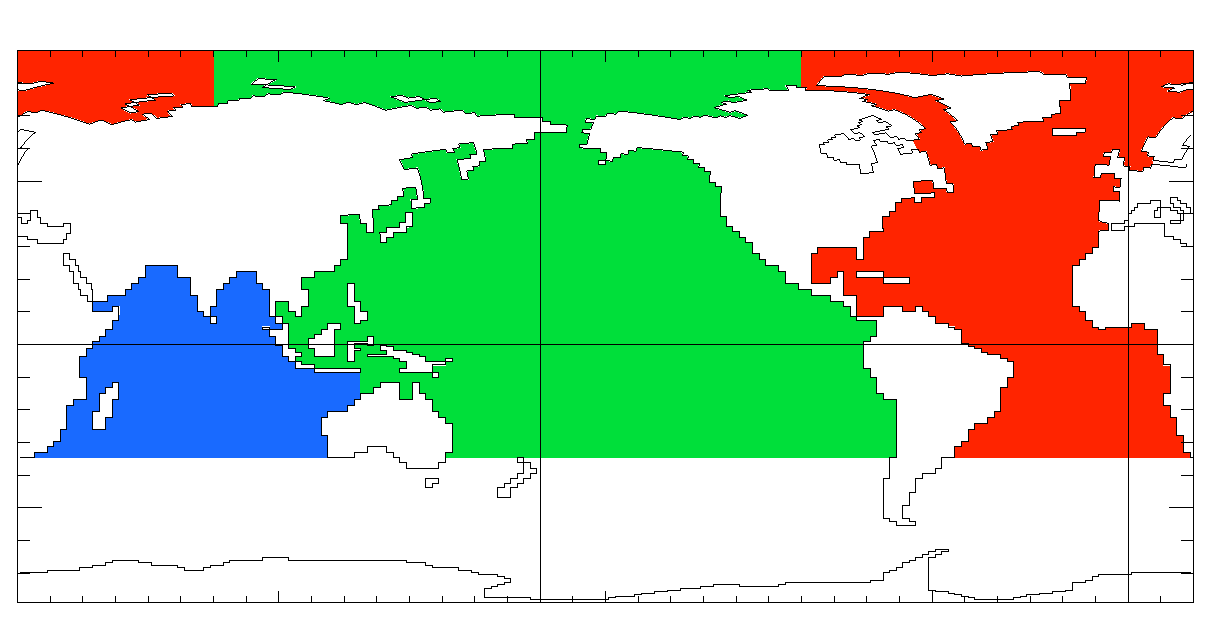
\includegraphics[width=1.0\textwidth]{./TexFiles/Figures/Fig_mask_subasins.pdf}
\caption{	\label{Fig_mask_subasins}
Decomposition of the World Ocean (here ORCA2) into sub-basin used in to compute
the heat and salt transports as well as the meridional stream-function: Atlantic basin (red), 
Pacific basin (green), Indian basin (bleue), Indo-Pacific basin (bleue+green). 
Note that semi-enclosed seas (Red, Med and Baltic seas) as well as Hudson Bay 
are removed from the sub-basins. Note also that the Arctic Ocean has been split 
into Atlantic and Pacific basins along the North fold line.  }
\end{center}   \end{figure}  
%>>>>>>>>>>>>>>>>>>>>>>>>>>>>

In addition, a series of diagnostics has been added in the \mdl{diaar5}. 
They corresponds to outputs that are required for AR5 simulations 
(see Section \ref{DIA_steric} below for one of them). 
Activating those outputs requires to define the \key{diaar5} CPP key.
\\
\\



% ================================================================
% Steric effect in sea surface height
% ================================================================
\section{Diagnosing the Steric effect in sea surface height}
\label{DIA_steric}


Changes in steric sea level are caused when changes in the density of the water 
column imply an expansion or contraction of the column. It is essentially produced 
through surface heating/cooling and to a lesser extent through non-linear effects of 
the equation of state (cabbeling, thermobaricity...).
Non-Boussinesq models contain all ocean effects within the ocean acting 
on the sea level. In particular, they include the steric effect. In contrast, 
Boussinesq models, such as \NEMO, conserve volume, rather than mass, 
and so do not properly represent expansion or contraction. The steric effect is 
therefore not explicitely represented.
This approximation does not represent a serious error with respect to the flow field 
calculated by the model \citep{Greatbatch_JGR94}, but extra attention is required
when investigating sea level, as steric changes are an important 
contribution to local changes in sea level on seasonal and climatic time scales.
This is especially true for investigation into sea level rise due to global warming. 

Fortunately, the steric contribution to the sea level consists of a spatially uniform 
component that can be diagnosed by considering the mass budget of the world 
ocean \citep{Greatbatch_JGR94}. 
In order to better understand how global mean sea level evolves and thus how
the steric sea level can be diagnosed, we compare, in the following, the 
non-Boussinesq and Boussinesq cases.

Let denote 
$\mathcal{M}$ the total mass of liquid seawater ($\mathcal{M}=\int_D \rho dv$), 
$\mathcal{V}$ the total volume of seawater ($\mathcal{V}=\int_D dv$), 
$\mathcal{A}$ the total surface of the ocean ($\mathcal{A}=\int_S ds$), 
$\bar{\rho}$ the global mean seawater (\textit{in situ}) density ($\bar{\rho}= 1/\mathcal{V} \int_D \rho \,dv$), and
$\bar{\eta}$ the global mean sea level ($\bar{\eta}=1/\mathcal{A}\int_S \eta \,ds$).

A non-Boussinesq fluid conserves mass. It satisfies the following relations:
\begin{equation} \label{Eq_MV_nBq} 
\begin{split} 
\mathcal{M} &=  \mathcal{V}  \;\bar{\rho}      	\\
\mathcal{V} &=  \mathcal{A}  \;\bar{\eta}	
\end{split}
\end{equation}
Temporal changes in total mass is obtained from the density conservation equation :
\begin{equation}  \label{Eq_Co_nBq}
\frac{1}{e_3} \partial_t ( e_3\,\rho) + \nabla( \rho \, \textbf{U} ) = \left. \frac{\textit{emp}}{e_3}\right|_\textit{surface}
\end{equation}
where $\rho$ is the \textit{in situ} density, and \textit{emp} the surface mass 
exchanges with the other media of the Earth system (atmosphere, sea-ice, land). 
Its global averaged leads to the total mass change 
\begin{equation}  \label{Eq_Mass_nBq}
\partial_t \mathcal{M} = \mathcal{A} \;\overline{\textit{emp}}
\end{equation}
where $\overline{\textit{emp}}=\int_S \textit{emp}\,ds$ is the net mass flux 
through the ocean surface.
Bringing \eqref{Eq_Mass_nBq} and the time derivative of \eqref{Eq_MV_nBq} 
together leads to the evolution equation of the mean sea level
\begin{equation} \label{Eq_ssh_nBq}
  \partial_t \bar{\eta} =  \frac{\overline{\textit{emp}}}{ \bar{\rho}} 
  					- \frac{\mathcal{V}}{\mathcal{A}}  \;\frac{\partial_t \bar{\rho} }{\bar{\rho}}
\end{equation}
The first term in equation \eqref{Eq_ssh_nBq} alters sea level by adding or 
subtracting mass from the ocean. 
The second term arises from temporal changes in the global mean 
density; $i.e.$ from steric effects. 

In a Boussinesq fluid, $\rho$ is replaced by $\rho_o$ in all the equation except when $\rho$ 
appears multiplied by the gravity ($i.e.$ in the hydrostatic balance of the primitive Equations). 
In particular, the mass conservation equation, \eqref{Eq_Co_nBq}, degenerates into 
the incompressibility equation:
\begin{equation}  \label{Eq_Co_Bq}
\frac{1}{e_3} \partial_t ( e_3 ) + \nabla( \textbf{U} ) =  \left. \frac{\textit{emp}}{\rho_o \,e_3}\right|_ \textit{surface}
\end{equation}
and the global average of this equation now gives the temporal change of the total volume,
\begin{equation}  \label{Eq_V_Bq}
  \partial_t \mathcal{V} =   \mathcal{A} \;\frac{\overline{\textit{emp}}}{\rho_o} 
\end{equation}
Only the volume is conserved, not mass, or, more precisely, the mass which is conserved is the 
Boussinesq mass, $\mathcal{M}_o = \rho_o \mathcal{V}$. The total volume (or equivalently  
the global mean sea level) is altered only by net volume fluxes across the ocean surface,  
not by changes in mean mass of the ocean: the steric effect is missing in a Boussinesq fluid.
 
Nevertheless, following \citep{Greatbatch_JGR94}, the steric effect on the volume can be 
diagnosed by considering the mass budget of the ocean. 
The apparent changes in $\mathcal{M}$, mass of the ocean, which are not induced by surface 
mass flux must be compensated by a spatially uniform change in the mean sea level due to 
expansion/contraction of the ocean \citep{Greatbatch_JGR94}. In others words, the Boussinesq 
mass, $\mathcal{M}_o$, can be related to $\mathcal{M}$, the  total mass of the ocean seen 
by the Boussinesq model, via the steric contribution to the sea level, $\eta_s$, a spatially 
uniform variable, as follows:
\begin{equation}  \label{Eq_M_Bq}
   \mathcal{M}_o  =  \mathcal{M} + \rho_o \,\eta_s \,\mathcal{A} 
\end{equation}
Any change in $\mathcal{M}$ which cannot be explained by the net mass flux through 
the ocean surface is converted into a mean change in sea level. Introducing the total density 
anomaly, $\mathcal{D}= \int_D d_a \,dv$, where $d_a= (\rho -\rho_o ) / \rho_o$  
is the density anomaly used in \NEMO (cf. \S\ref{TRA_eos}) in \eqref{Eq_M_Bq}
leads to a very simple form for the steric height:
\begin{equation}  \label{Eq_steric_Bq}
   \eta_s = - \frac{1}{\mathcal{A}} \mathcal{D} 
\end{equation}

The above formulation of the steric height of a Boussinesq ocean requires four remarks.
First, one can be tempted to define $\rho_o$ as the initial value of $\mathcal{M}/\mathcal{V}$,
$i.e.$ set $\mathcal{D}_{t=0}=0$, so that the initial steric height is zero. We do not
recommend that. Indeed, in this case $\rho_o$ depends on the initial state of the ocean. 
Since $\rho_o$ has a direct effect on the dynamics of the ocean (it appears in the pressure 
gradient term of the momentum equation) it is definitively not a good idea when 
inter-comparing experiments. 
We better recommend to fixe once for all $\rho_o$ to $1035\;Kg\,m^{-3}$. This value is a 
sensible choice for the reference density used in a Boussinesq ocean climate model since, 
with the exception of only a small percentage of the ocean, density in the World Ocean 
varies by no more than 2$\%$ from this value (\cite{Gill1982}, page 47).

Second, we have assumed here that the total ocean surface, $\mathcal{A}$, does not
change when the sea level is changing as it is the case in all global ocean GCMs 
(wetting and drying of grid point is not allowed). 
  
Third, the discretisation of \eqref{Eq_steric_Bq} depends on the type of free surface
which is considered. In the non linear free surface case, $i.e.$ \key{vvl} defined, it is
given by
\begin{equation}  \label{Eq_discrete_steric_Bq}
   \eta_s =  - \frac{ \sum_{i,\,j,\,k} d_a\; e_{1t} e_{2t} e_{3t} }
   					{ \sum_{i,\,j,\,k}         e_{1t} e_{2t} e_{3t} } 
\end{equation}
whereas in the linear free surface, the volume above the \textit{z=0} surface must be explicitly taken 
into account to better approximate the total ocean mass and thus the steric sea level:
\begin{equation}  \label{Eq_discrete_steric_Bq}
   \eta_s =  - \frac{ \sum_{i,\,j,\,k} d_a\; e_{1t}e_{2t}e_{3t} + \sum_{i,\,j} d_a\; e_{1t}e_{2t} \eta }
   						{\sum_{i,\,j,\,k} e_{1t}e_{2t}e_{3t} + \sum_{i,\,j}           e_{1t}e_{2t} \eta } 
\end{equation}

The fourth and last remark concerns the effective sea level and the presence of sea-ice.
In the real ocean, sea ice (and snow above it)  depresses the liquid seawater through 
its mass loading. This depression is a result of the mass of sea ice/snow system acting 
on the liquid ocean. There is, however, no dynamical effect associated with these depressions 
in the liquid ocean sea level, so that there are no associated ocean currents. Hence, the 
dynamically relevant sea level is the effective sea level, $i.e.$ the sea level as if sea ice 
(and snow) were converted to liquid seawater \citep{Campin_al_OM08}. However,
in the current version of \NEMO the sea-ice is levitating above the ocean without 
mass exchanges between ice and ocean. Therefore the model effective sea level
is always given by $\eta + \eta_s$, whether or not there is sea ice present.

In AR5 outputs, the thermosteric sea level is demanded. It is steric sea level due to 
changes in ocean density arising just from changes in temperature. It is given by:
\begin{equation}  \label{Eq_thermosteric_Bq}
   \eta_s = - \frac{1}{\mathcal{A}} \int_D d_a(T,S_o,p_o) \,dv
\end{equation}
where $S_o$ and $p_o$ are the initial salinity and pressure, respectively.

Both steric and thermosteric sea level are computed in \mdl{diaar5} which needs
the \key{diaar5} defined to be called.

% ================================================================












